\section{Zusammenfassung und Diskussion}

In Versuch 255 untersuchten wir unter Einsatz der Drehkristallmethode mit einem LiF- und einem NaCl-Kristall das Spektrum der Röntgenstrahlung einer Röntgenröhre mit Molybdänanode. Das Röntgenspektrum zeichnet sich durch ein kontinuierliches Spektrum aus, welches durch Bremsstrahlung erzeugt wird, dem ein diskretes Spektrum, erzeugt durch Ionisation im Anodenmaterial der Röntgenröhre, überlagert ist.

Wir untersuchten zunächst das Röntgengenspektrum, aufgezeichnet in der Drehkristallmethode mit einem LiF-Kristall. Dieses ist noch einmal in \abbref{fig:spektrum_lif_komplett_zsmf} abgebildet.

\begin{figure}[H]
  \centering
  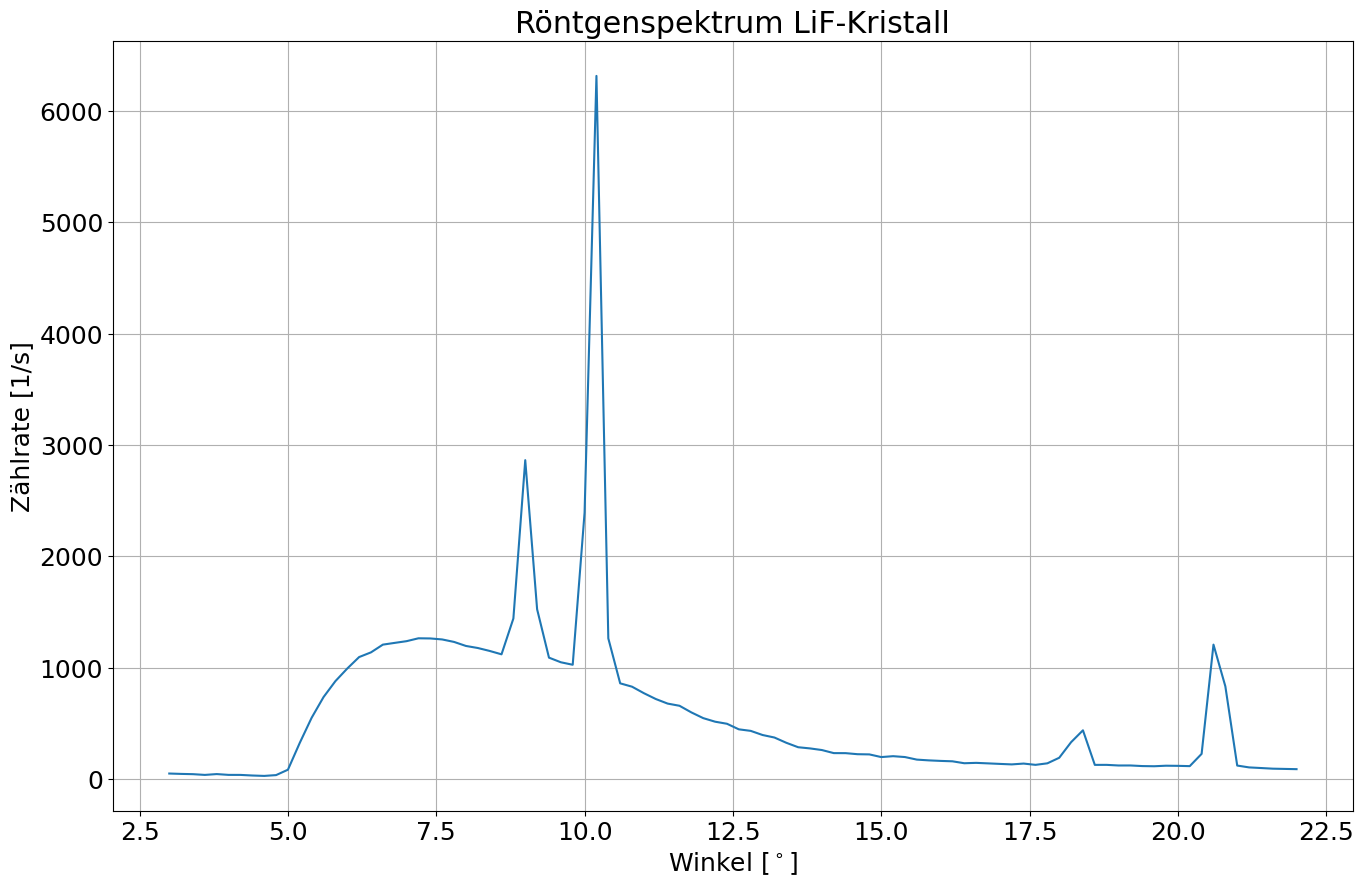
\includegraphics[width=.9\textwidth]{files/plots/spektrum_lif_komplett.png}
  \caption{Röntgenspektrum mit LiF-Kristall}
  \label{fig:spektrum_lif_komplett_zsmf}
\end{figure}

Im ersten Teil bestimmten wir die Grenzwellenlänge des Spektrums, also den Punkt am kurzwelligen Ende, an dem das Spektrum erster Ordnung einsetz. Hierzu ermittelten wir einen Wert von
\begin{align}
  \lambda_{Grenz} = (34.33 \pm 3.08) \si{\pico\meter}.
\end{align}

Aus der Grenzwellenlänge berechneten wir für das Planck'sche Wirkungsquantum einen Wert von
\begin{align}
  h = (6.4 \pm 0.6) \cdot 10^{-34} \si{\joule\second}.
\end{align}

Dieser Wert weicht von dem in der Praktikumsanleitung gegebenen Wert von $h_{lit} = 6.6261 \cdot 10^{-34} \si{\joule\second}$ um $0.36\sigma$ ab. Diese Abweichung ist sehr gering und kann als nicht signifikant angesehen werden.

Am Ende dieses Aufgabenteils bestimmten wir noch den Winkel des Drehkristalls, ab dem das Spektrum zweiter Ordnung einsetzt. Hierfür kamen wir auf einen Wert von
\begin{align}
  \vartheta_{0,2. Ord} = (9.813 \pm 0.016)\si{\degree}.
\end{align}

Im zweiten Versuchsteil betrachteten wir die Lagen der $K_{\alpha}$- und $K_{\beta}$-Linien erster und zweiter Ordnung, welch durch Ionisation in der Molybdänanode erzeugt werden, genauer. Für alle vier Linien bestimmten wir mittels eines Fits einer Gaußkurve an die Daten die Winkelposition des Drehkristalls, an welcher diese auftreten, die zugehörige Standardabweichung, sowie deren Halbwertsbreite. Mithilfe des Bragg'schen Gesetztes berechneten wir aus den Winkeln wieder die zugehörigen Wellenlängen und bildeten einen Mittelwert über die Linien erster und zweiter Ordnung. Die Ergebnisse sind noch einmal in \tabref{tab:k_linien_zsmf} zusammengefasst. Die Literaturwerte für die Positionen der Linien stammen ebenfalls aus der Praktikumsanleitung.

\begin{table}[H]
  \centering
  \begin{tabular}{c|c|c|c|c|c}
    Linie & Ordnung & $\lambda$ $[\si{\pico\meter}]$ & $\overline{\lambda}$ $[\si{\pico\meter}]$ & $\lambda_{Lit}$ $[\si{\pico\meter}]$ & Abweichung\\\hline
    %
    \multirow{2}{*}{$K_\alpha$} & 1 & $71.27 \pm 0.04$ & \multirow{2}{*}{$71.171 \pm 0.018$} & \multirow{2}{*}{$71.1$} & \multirow{2}{*}{$x\sigma$}\\
     & 2 & $71.074 \pm 0.011$ & & & \\\hline
    %
    %
    \multirow{2}{*}{$K_\beta$} & 1 & $63.27 \pm 0.05$ & \multirow{2}{*}{$63.274 \pm 0.029$} & \multirow{2}{*}{$63.1$} & \multirow{2}{*}{$x\sigma$}\\
     & 2 & $63.27 \pm 0.04$ & & & 
  \end{tabular}
  \label{tab:k_linien_zsmf}
\end{table}